\chapter{Dentro do átomo}\label{ch:g9:inside-the-atom}

Em 1909, num laboratório em Manchester, um feixe de partículas minúsculas
e rápidas foi disparado contra uma folha de ouro com algumas centenas de
\omterm{def:g7:atoms-and-molecules:atom}{átomos} de espessura. Quase todas atravessaram em linha reta, como se o
ouro fosse vazio. Mas cerca de uma em vários milhares voltou para trás.
``Foi como se você disparasse um projétil de 15 polegadas contra uma
folha de papel de seda e ele voltasse e atingisse você'', disse Ernest
Rutherford, cujos alunos tinham feito o experimento. O \omterm{def:g7:atoms-and-molecules:atom}{átomo}, o pedaço
indivisível da matéria, tinha uma estrutura --- e era quase
inteiramente vazio.

\begin{recall}
Toda a matéria é feita de \omterm{def:g7:atoms-and-molecules:atom}{átomos}, de cerca de cem tipos diferentes, cada
um com um símbolo como \ce{H}, \ce{C}, \ce{O}, \ce{Fe}. Os \omterm{def:g7:atoms-and-molecules:atom}{átomos} se
juntam em \omterm{def:g7:atoms-and-molecules:molecule}{moléculas}, descritas por fórmulas como \ce{H2O}
(\cref{ch:g7:atoms-and-molecules}).
\end{recall}

\section{Núcleo e elétrons}

\begin{definition}[Núcleo e elétron]\label{def:g9:inside-the-atom:nucleus}
Todo \omterm{def:g7:atoms-and-molecules:atom}{átomo} tem um centro minúsculo e pesado, o
\emph{núcleo}\index{nucleo@núcleo}, que tem carga elétrica positiva. Em volta
dele se movem partículas muito mais leves, os
\emph{elétrons}\index{eletron@elétron}, cada um com a mesma carga negativa,
$-e$.
\end{definition}

\begin{proposition}[Um átomo é neutro]\label{prop:g9:inside-the-atom:neutral}
% ledger: const:e
Um \omterm{def:g7:atoms-and-molecules:atom}{átomo}, como um todo, não tem carga elétrica: a carga positiva do
\omterm{def:g9:inside-the-atom:nucleus}{núcleo} é compensada exatamente pelas cargas negativas dos \omterm{def:g9:inside-the-atom:nucleus}{elétrons}. A
carga $e$ é minúscula: $e = \qty{1.60e-19}{C}$ (o coulomb, unidade de
carga, pertence ao livro de física).
\end{proposition}

\begin{omfigure}
\begin{tikzpicture}[font=\small]
  \shade[inner color=omDef!35, outer color=white] (0,0) circle (2.2);
  \draw[omDef!60, dashed] (0,0) circle (2.2);
  \foreach \a/\r in {20/1.6,95/1.1,150/1.9,215/1.4,290/1.7,340/0.9} {
    \fill[omDef] (\a:\r) circle (0.06);
    \node[font=\scriptsize, omDef] at ($(\a:\r)+(0.18,0.16)$) {$-$};
  }
  \fill[red!70!black] (0,0) circle (0.1);
  \draw[<-, omProp, thick] (-0.12,0.02) -- (-3.0,0.9) node[left, text=black, align=right]
    {núcleo: minúsculo,\\ pesado, positivo};
  \draw[<-, omProp, thick] ($(20:1.6)+(0.08,0.02)$) -- (3.0,0.9) node[right, text=black]
    {um elétron: leve, negativo};
  \draw[<-, omProp, thick] (300:2.2) -- (3.0,-1.4) node[right, text=black, align=left]
    {os elétrons se movem numa nuvem\\ em volta do núcleo};
\end{tikzpicture}

{\small Um \omterm{def:g7:atoms-and-molecules:atom}{átomo}, fora de escala. Se o \omterm{def:g9:inside-the-atom:nucleus}{núcleo} fosse desenhado do tamanho
do ponto vermelho, a nuvem de \omterm{def:g9:inside-the-atom:nucleus}{elétrons} teria algumas centenas de metros
de diâmetro.}
\end{omfigure}

\section{Prótons e nêutrons}

\begin{definition}[Próton, nêutron, núcleon]\label{def:g9:inside-the-atom:proton}
O \omterm{def:g9:inside-the-atom:nucleus}{núcleo} é formado por dois tipos de partículas: os
\emph{prótons}\index{proton@próton}, cada um com a carga $+e$, e os
\emph{nêutrons}\index{neutron@nêutron}, que não têm carga. Os prótons e os
nêutrons, que têm quase a mesma massa, são chamados juntos de
\emph{núcleons}\index{nucleon@núcleon}.
\end{definition}

\begin{definition}[Número atômico e número de massa]\label{def:g9:inside-the-atom:atomic-number}
O número de \omterm{def:g9:inside-the-atom:proton}{prótons} de um \omterm{def:g9:inside-the-atom:nucleus}{núcleo} é o \emph{número
atômico}\index{numero atomico@número atômico}, representado por $Z$. O número de
\omterm{def:g9:inside-the-atom:proton}{núcleons} (\omterm{def:g9:inside-the-atom:proton}{prótons} e \omterm{def:g9:inside-the-atom:proton}{nêutrons} juntos) é o \emph{número de
massa}\index{numero de massa@número de massa}, representado por $A$. O número de
\omterm{def:g9:inside-the-atom:proton}{nêutrons} é $N = A - Z$.
\end{definition}

\begin{notation}[O símbolo do nuclídeo]\label{not:g9:inside-the-atom:symbol}
Um \omterm{def:g7:atoms-and-molecules:atom}{átomo} com um dado \omterm{def:g9:inside-the-atom:nucleus}{núcleo} é escrito com o seu símbolo, o \omterm{def:g9:inside-the-atom:atomic-number}{número de
massa} no alto à esquerda e o \omterm{def:g9:inside-the-atom:atomic-number}{número atômico} embaixo à esquerda:
\ce{^{A}_{Z}X}. Por exemplo, \ce{^{12}_{6}C} tem 6 \omterm{def:g9:inside-the-atom:proton}{prótons} e $12 - 6 =
6$ \omterm{def:g9:inside-the-atom:proton}{nêutrons}; \ce{^{56}_{26}Fe} tem 26 \omterm{def:g9:inside-the-atom:proton}{prótons} e 30 \omterm{def:g9:inside-the-atom:proton}{nêutrons}.
\end{notation}

\begin{method}[Ler o símbolo de um nuclídeo]\label{met:g9:inside-the-atom:read}
Para \ce{^{A}_{Z}X}:
\begin{enumerate}
  \item \omterm{def:g9:inside-the-atom:proton}{prótons}: $Z$;
  \item \omterm{def:g9:inside-the-atom:proton}{nêutrons}: $A - Z$;
  \item \omterm{def:g9:inside-the-atom:nucleus}{elétrons} do \omterm{def:g7:atoms-and-molecules:atom}{átomo} neutro: $Z$, o mesmo número que os \omterm{def:g9:inside-the-atom:proton}{prótons}.
\end{enumerate}
Para \ce{^{23}_{11}Na}: 11 \omterm{def:g9:inside-the-atom:proton}{prótons}, 12 \omterm{def:g9:inside-the-atom:proton}{nêutrons}, 11 \omterm{def:g9:inside-the-atom:nucleus}{elétrons}.
\end{method}

\begin{omfigure}
\begin{tikzpicture}[font=\small]
  \node[font=\Huge, inner sep=1pt] (x) at (0,0) {\ce{^{35}_{17}Cl}};
  \draw[<-, omProp, thick, shorten <=3pt] ([xshift=5pt,yshift=-7pt]x.north west) -- (-2.6,1.0)
    node[left, text=black, align=right] {número de massa $A = 35$:\\ prótons + nêutrons};
  \draw[<-, omProp, thick, shorten <=3pt] ([xshift=5pt,yshift=7pt]x.south west) -- (-2.6,-1.0)
    node[left, text=black, align=right] {número atômico $Z = 17$:\\ prótons};
  \draw[<-, omProp, thick] ([xshift=2pt]x.east) -- (2.2,0) node[right, text=black,
    align=left] {símbolo do elemento:\\ cloro};
\end{tikzpicture}

{\small Ler o símbolo de um nuclídeo: este \omterm{def:g7:atoms-and-molecules:atom}{átomo} de cloro tem 17 \omterm{def:g9:inside-the-atom:proton}{prótons},
$35 - 17 = 18$ \omterm{def:g9:inside-the-atom:proton}{nêutrons} e, quando neutro, 17 \omterm{def:g9:inside-the-atom:nucleus}{elétrons}.}
\end{omfigure}

\section{O elemento químico e os seus isótopos}

\begin{definition}[Elemento químico]\label{def:g9:inside-the-atom:element}
Um \emph{elemento químico}\index{elemento quimico@elemento químico} é o conjunto de todos
os \omterm{def:g7:atoms-and-molecules:atom}{átomos}, e de todos os \omterm{def:g7:atoms-and-molecules:atom}{átomos} carregados formados a partir deles, que
têm o mesmo \omterm{def:g9:inside-the-atom:atomic-number}{número atômico} $Z$. Cada elemento tem um nome e um símbolo:
todo \omterm{def:g7:atoms-and-molecules:atom}{átomo} com 6 \omterm{def:g9:inside-the-atom:proton}{prótons} é um \omterm{def:g7:atoms-and-molecules:atom}{átomo} de carbono, \ce{C}; todo \omterm{def:g7:atoms-and-molecules:atom}{átomo} com 8
\omterm{def:g9:inside-the-atom:proton}{prótons} é um \omterm{def:g7:atoms-and-molecules:atom}{átomo} de oxigênio, \ce{O}.
\end{definition}

\begin{definition}[Isótopos]\label{def:g9:inside-the-atom:isotope}
\omterm{def:g7:atoms-and-molecules:atom}{Átomos} do mesmo elemento que têm números diferentes de \omterm{def:g9:inside-the-atom:proton}{nêutrons}, e
portanto \omterm{def:g9:inside-the-atom:atomic-number}{números de massa} diferentes, são \emph{isótopos}\index{isotopo@isótopo}
desse elemento. Eles têm o mesmo $Z$ e $A$ diferentes.
\end{definition}

\begin{example}[Isótopos do carbono e do hidrogênio]\label{ex:g9:inside-the-atom:isotopes}
% ledger: iso:C12, iso:C13, iso:H2
O carbono natural tem cerca de \qty{98.9}{\percent} de carbono-12,
\ce{^{12}_{6}C}, e \qty{1.1}{\percent} de carbono-13, \ce{^{13}_{6}C},
com um traço de carbono-14, \ce{^{14}_{6}C}, cuja lenta transformação
em outro \omterm{def:g9:inside-the-atom:nucleus}{núcleo} é usada para datar madeiras e ossos antigos (a
radioatividade pertence ao livro de física). O hidrogênio tem três
\omterm{def:g9:inside-the-atom:isotope}{isótopos}: \ce{^{1}_{1}H}, sem nenhum \omterm{def:g9:inside-the-atom:proton}{nêutron}, de longe o mais comum; o
deutério \ce{^{2}_{1}H}, alguns \omterm{def:g7:atoms-and-molecules:atom}{átomos} em cada cem mil; e o trítio
\ce{^{3}_{1}H}.
\end{example}

\begin{proposition}[Os isótopos se comportam igual na química]\label{prop:g9:inside-the-atom:alike}
A química de um \omterm{def:g7:atoms-and-molecules:atom}{átomo} depende dos seus \omterm{def:g9:inside-the-atom:nucleus}{elétrons}, e os \omterm{def:g9:inside-the-atom:isotope}{isótopos} de um
elemento têm o mesmo número de \omterm{def:g9:inside-the-atom:nucleus}{elétrons}. Os \omterm{def:g9:inside-the-atom:isotope}{isótopos} reagem, portanto,
do mesmo modo: a água feita com deutério tem o aspecto e o comportamento
quase exatamente iguais aos da água comum.
\end{proposition}

\begin{omfigure}
\begin{tikzpicture}[font=\small, p/.style={circle, inner sep=0pt, minimum size=4.2mm,
    ball color=red!65}, n/.style={circle, inner sep=0pt, minimum size=4.2mm,
    ball color=black!20}]
  \node[p] at (0,0) {};
  \node[anchor=north, align=center] at (0,-0.45) {\ce{^{1}_{1}H}\\ 1 próton};
  \node[p] at (3.0,0) {}; \node[n] at (3.35,0.1) {};
  \node[anchor=north, align=center] at (3.2,-0.45) {\ce{^{2}_{1}H}\\ 1 próton, 1 nêutron};
  \node[p] at (6.4,0) {}; \node[n] at (6.75,0.12) {}; \node[n] at (6.55,0.35) {};
  \node[anchor=north, align=center] at (6.6,-0.45) {\ce{^{3}_{1}H}\\ 1 próton, 2 nêutrons};
  \node[draw=black!30, fill=red!65, circle, minimum size=3mm, inner sep=0pt] at (9.1,0.2) {};
  \node[anchor=west] at (9.3,0.2) {próton};
  \node[draw=black!30, fill=black!20, circle, minimum size=3mm, inner sep=0pt] at (9.1,-0.3) {};
  \node[anchor=west] at (9.3,-0.3) {nêutron};
\end{tikzpicture}

{\small Os \omterm{def:g9:inside-the-atom:nucleus}{núcleos} dos três \omterm{def:g9:inside-the-atom:isotope}{isótopos} do hidrogênio: um \omterm{def:g9:inside-the-atom:proton}{próton} cada, e 0,
1 ou 2 \omterm{def:g9:inside-the-atom:proton}{nêutrons}.}
\end{omfigure}

\section{Tamanhos e massas}

\begin{proposition}[O núcleo é minúsculo e contém quase toda a massa]\label{prop:g9:inside-the-atom:sizes}
% ledger: const:a0, r:proton, const:mp, const:mn, const:me
Um \omterm{def:g7:atoms-and-molecules:atom}{átomo} mede cerca de \qty{e-10}{m} de diâmetro; o seu \omterm{def:g9:inside-the-atom:nucleus}{núcleo}, de
\qty{e-15}{m} a \qty{e-14}{m}: algo entre dez mil e cem mil vezes menor.
As massas das partículas são
\[
  m_p = \qty{1.673e-27}{kg},\qquad m_n = \qty{1.675e-27}{kg},\qquad
  m_e = \qty{9.11e-31}{kg}.
\]
Um \omterm{def:g9:inside-the-atom:proton}{próton} é cerca de 1836 vezes mais pesado do que um \omterm{def:g9:inside-the-atom:nucleus}{elétron}, por isso
mais de \qty{99.9}{\percent} da massa de um \omterm{def:g7:atoms-and-molecules:atom}{átomo} está no \omterm{def:g9:inside-the-atom:nucleus}{núcleo}.
\end{proposition}

\begin{example}[Uma bolinha de gude num estádio]\label{ex:g9:inside-the-atom:marble}
Se o \omterm{def:g9:inside-the-atom:nucleus}{núcleo} de um \omterm{def:g7:atoms-and-molecules:atom}{átomo} fosse uma bolinha de gude de \qty{1}{cm} de
diâmetro, o \omterm{def:g7:atoms-and-molecules:atom}{átomo} teria cerca de
$\qty{1}{cm} \times 100\,000 = \qty{1}{km}$ de diâmetro: uma bolinha de
gude no meio de um estádio enorme, com alguns grãozinhos de poeira ---
os \omterm{def:g9:inside-the-atom:nucleus}{elétrons} --- girando em volta das arquibancadas. A matéria é
principalmente espaço vazio.
\end{example}

\begin{method}[A massa de um átomo]\label{met:g9:inside-the-atom:mass}
Como os \omterm{def:g9:inside-the-atom:proton}{prótons} e os \omterm{def:g9:inside-the-atom:proton}{nêutrons} têm quase a mesma massa e os \omterm{def:g9:inside-the-atom:nucleus}{elétrons} são
muito leves, a massa de um \omterm{def:g7:atoms-and-molecules:atom}{átomo} é próxima de $A \times
\qty{1.67e-27}{kg}$, em que $A$ é o seu \omterm{def:g9:inside-the-atom:atomic-number}{número de massa}. Um \omterm{def:g7:atoms-and-molecules:atom}{átomo} de
carbono-12:
$12 \times 1.67 \times 10^{-27} = \qty{2.00e-26}{kg}$.
\end{method}

\section{Uma breve história do modelo atômico}

\begin{history}[Do indivisível ao núcleo, 1897--1932]
Em 1897, J.~J.~Thomson descobriu o \omterm{def:g9:inside-the-atom:nucleus}{elétron}, uma partícula muito mais leve
do que qualquer \omterm{def:g7:atoms-and-molecules:atom}{átomo}: afinal, os \omterm{def:g7:atoms-and-molecules:atom}{átomos} podiam ser divididos. Ele
imaginou o \omterm{def:g7:atoms-and-molecules:atom}{átomo} como uma bola de matéria positiva salpicada de
\omterm{def:g9:inside-the-atom:nucleus}{elétrons}. Em 1909--1911, o experimento da folha de ouro da equipe de
Rutherford mostrou que a carga positiva e quase toda a massa estão num
\omterm{def:g9:inside-the-atom:nucleus}{núcleo} minúsculo. Em 1913, Niels Bohr propôs que os \omterm{def:g9:inside-the-atom:nucleus}{elétrons} ocupam
níveis de energia fixos em volta dele, e em 1932 James Chadwick
descobriu o \omterm{def:g9:inside-the-atom:proton}{nêutron}.
\end{history}

\begin{omfigure}
\begin{minipage}[b]{0.3\linewidth}\centering
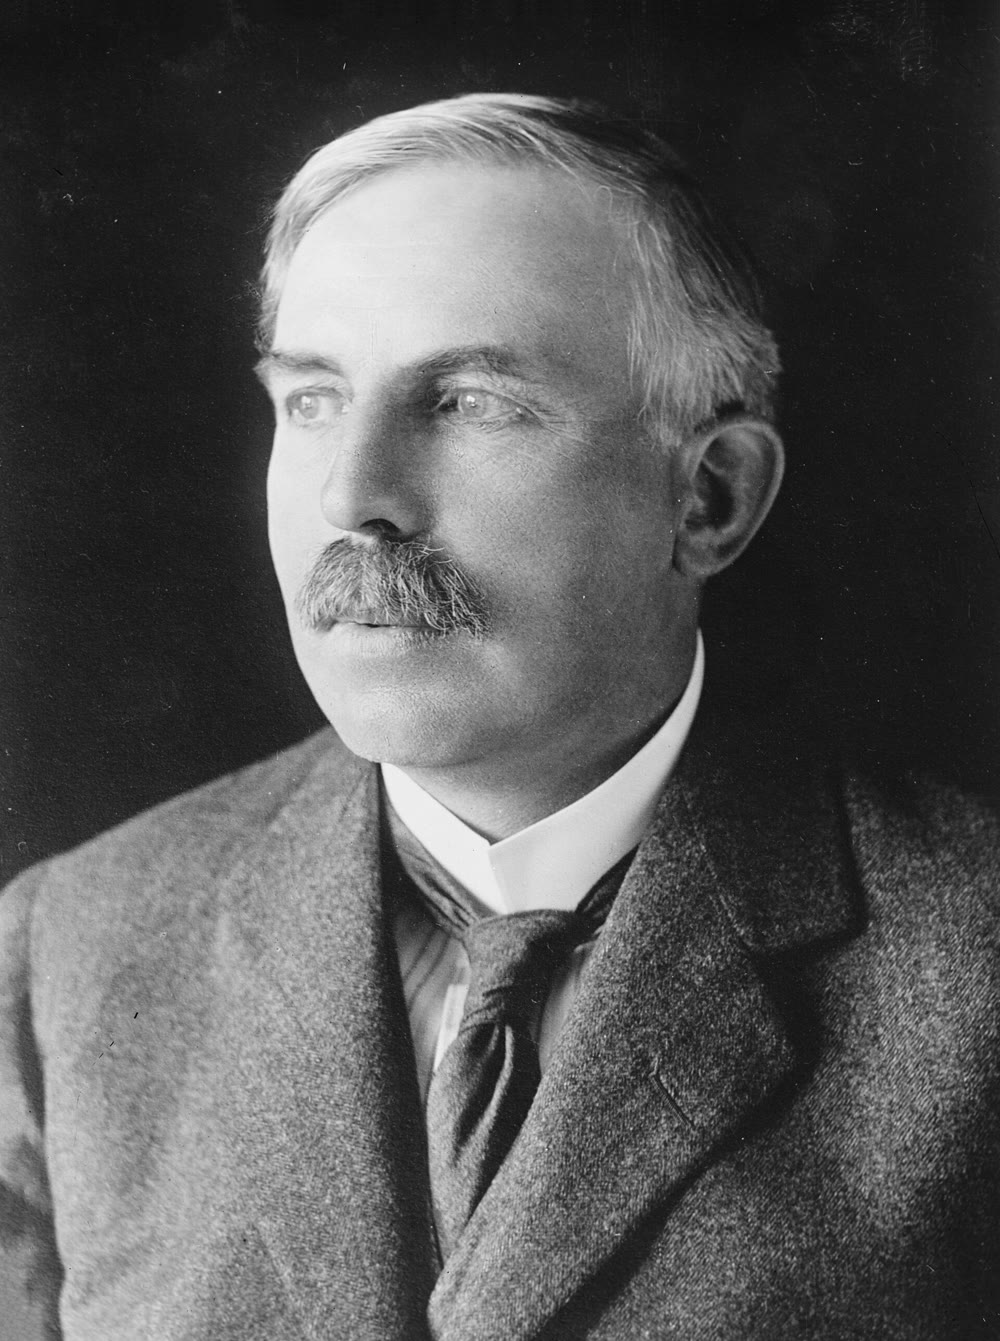
\includegraphics[width=\linewidth]{images/book1/rutherford.jpg}

{\small Ernest Rutherford (1871--1937).}
\end{minipage}\hfill
\begin{minipage}[b]{0.66\linewidth}\centering
\begin{tikzpicture}[font=\small]
  \fill[black!45] (0,-0.5) rectangle (0.9,0.5);
  \node[anchor=north, align=center] at (0.45,-0.55) {fonte de\\ partículas alfa};
  \draw[->, thick, red!70!black] (0.9,0) -- (2.8,0);
  \fill[yellow!70!orange] (2.8,-1.6) rectangle (2.88,1.6);
  \node[anchor=north] at (2.84,-1.65) {folha de ouro};
  \draw[omDef!40, line width=4pt] (5.6,-1.8) arc[start angle=-30, end angle=30, radius=3.6];
  \foreach \y in {-0.3,-0.1,0.1,0.3} \draw[->, red!70!black] (2.88,\y) -- (5.3,\y);
  \draw[->, red!70!black] (2.88,0.05) -- (5.0,1.15);
  \draw[->, red!70!black] (2.88,-0.05) -- (4.9,-1.3);
  \draw[->, red!70!black, thick] (2.8,0.02) .. controls (2.2,0.35) .. (1.6,0.95);
  \node[anchor=west, align=left, font=\footnotesize] at (6.25,0) {a maioria\\ atravessa\\ em linha reta};
  \node[anchor=south, align=center, font=\footnotesize] at (1.6,1.0) {pouquíssimas\\ voltam para trás};
\end{tikzpicture}

{\small O experimento da folha de ouro: a maioria das partículas
atravessa em linha reta; algumas são desviadas; pouquíssimas voltam
para trás ao bater num \omterm{def:g9:inside-the-atom:nucleus}{núcleo}.}
\end{minipage}
\end{omfigure}

\section{Exercícios}

\begin{exercise}[$\star$]\label{exo:g9:inside-the-atom:1}
Dê o nome das partículas do \omterm{def:g9:inside-the-atom:nucleus}{núcleo} e das partículas em volta dele, com o
sinal da carga de cada uma.
\end{exercise}

\begin{exercise}[$\star$]\label{exo:g9:inside-the-atom:2}
Dê o número de \omterm{def:g9:inside-the-atom:proton}{prótons}, de \omterm{def:g9:inside-the-atom:proton}{nêutrons} e de \omterm{def:g9:inside-the-atom:nucleus}{elétrons} de \ce{^{16}_{8}O},
\ce{^{27}_{13}Al} e \ce{^{40}_{20}Ca}.
\end{exercise}

\begin{exercise}[$\star$]\label{exo:g9:inside-the-atom:3}
Por que um \omterm{def:g7:atoms-and-molecules:atom}{átomo} é eletricamente neutro?
\end{exercise}

\begin{exercise}[$\star$]\label{exo:g9:inside-the-atom:4}
Um \omterm{def:g7:atoms-and-molecules:atom}{átomo} tem 26 \omterm{def:g9:inside-the-atom:proton}{prótons} e 30 \omterm{def:g9:inside-the-atom:proton}{nêutrons}. Escreva o símbolo do nuclídeo
(o elemento é o ferro, \ce{Fe}).
\end{exercise}

\begin{exercise}[$\star\star$]\label{exo:g9:inside-the-atom:5}
\ce{^{35}_{17}Cl} e \ce{^{37}_{17}Cl} são o mesmo elemento? São
\omterm{def:g9:inside-the-atom:isotope}{isótopos}? Explique.
\end{exercise}

\begin{exercise}[$\star\star$]\label{exo:g9:inside-the-atom:6}
\ce{^{14}_{6}C} e \ce{^{14}_{7}N} são \omterm{def:g9:inside-the-atom:isotope}{isótopos}? Explique.
\end{exercise}

\begin{exercise}[$\star\star$]\label{exo:g9:inside-the-atom:7}
Calcule, em notação científica, a massa aproximada de um \omterm{def:g7:atoms-and-molecules:atom}{átomo} de
\ce{^{56}_{26}Fe}.
\end{exercise}

\begin{exercise}[$\star\star$]\label{exo:g9:inside-the-atom:8}
No experimento da folha de ouro, por que a maioria das partículas
atravessa o ouro em linha reta?
\end{exercise}

\begin{exercise}[$\star\star$]\label{exo:g9:inside-the-atom:9}
Quantas vezes um \omterm{def:g9:inside-the-atom:nucleus}{núcleo} de \qty{e-15}{m} é menor do que um \omterm{def:g7:atoms-and-molecules:atom}{átomo}
(\qty{e-10}{m})? Escreva a resposta como uma potência de dez.
\end{exercise}

\begin{exercise}[$\star\star$]\label{exo:g9:inside-the-atom:10}
Por que os \omterm{def:g9:inside-the-atom:isotope}{isótopos} de um elemento têm a mesma química?
\end{exercise}

\begin{exercise}[$\star\star\star$]\label{exo:g9:inside-the-atom:11}
Um \omterm{def:g7:atoms-and-molecules:atom}{átomo} de ferro tem 26 \omterm{def:g9:inside-the-atom:nucleus}{elétrons}. Calcule a massa total deles, e depois
a fração da massa de um \omterm{def:g7:atoms-and-molecules:atom}{átomo} de \ce{^{56}_{26}Fe} que eles representam
(use a massa encontrada no exercício~7).
\end{exercise}

\begin{exercise}[$\star\star\star$]\label{exo:g9:inside-the-atom:12}
% ledger: iso:Cu63, iso:Cu65
O cobre natural tem \qty{69.15}{\percent} de cobre-63 e
\qty{30.85}{\percent} de cobre-65. Entre 10\,000 \omterm{def:g7:atoms-and-molecules:atom}{átomos} de cobre,
quantos são de cada \omterm{def:g9:inside-the-atom:isotope}{isótopo}? Qual é o número médio de \omterm{def:g9:inside-the-atom:proton}{núcleons} por
\omterm{def:g7:atoms-and-molecules:atom}{átomo} de cobre?
\end{exercise}

\clearpage % mantém o título junto da caixa do problema (ele tinha ficado isolado no pé de uma página)
\section{Problema: pesar o cloro}

\begin{problem}[{Problema de fim de semana --- dois isótopos do cloro, a
massa de cada átomo e a massa média de um átomo de cloro}]
\label{pb:g9:inside-the-atom:1}
% ledger: iso:Cl35, iso:Cl37, const:me, const:mp, const:mn
O cloro natural é uma \omterm{def:g6:pure-substances-and-mixtures:mixture}{mistura} de dois \omterm{def:g9:inside-the-atom:isotope}{isótopos}, o cloro-35 e o cloro-37:
de cada 1000 \omterm{def:g7:atoms-and-molecules:atom}{átomos} de cloro, cerca de 758 são de cloro-35 e 242 de
cloro-37. Tome a massa de um \omterm{def:g9:inside-the-atom:proton}{núcleon} como \qty{1.67e-27}{kg} e a massa
de um \omterm{def:g9:inside-the-atom:nucleus}{elétron} como \qty{9.11e-31}{kg}. O \omterm{def:g9:inside-the-atom:atomic-number}{número atômico} do cloro é 17.

\medskip
\noindent\textbf{Parte I --- Dois \omterm{def:g9:inside-the-atom:nucleus}{núcleos}.}
\begin{enumerate}
  \item Escreva os símbolos dos nuclídeos dos dois \omterm{def:g9:inside-the-atom:isotope}{isótopos}.
  \item Dê o número de \omterm{def:g9:inside-the-atom:proton}{prótons}, de \omterm{def:g9:inside-the-atom:proton}{nêutrons} e de \omterm{def:g9:inside-the-atom:nucleus}{elétrons} de cada um.
  \item Por que os dois se chamam cloro? Por que eles são \omterm{def:g9:inside-the-atom:isotope}{isótopos}?
  \item Uma amostra de cloro-37 vai reagir com o sódio do mesmo modo que
        uma amostra de cloro-35? Explique.
\end{enumerate}

\medskip
\noindent\textbf{Parte II --- A massa de cada \omterm{def:g7:atoms-and-molecules:atom}{átomo}.}
\begin{enumerate}[resume]
  \item Calcule a massa do \omterm{def:g9:inside-the-atom:nucleus}{núcleo} de um \omterm{def:g7:atoms-and-molecules:atom}{átomo} de cloro-35.
  \item Calcule a massa dos 17 \omterm{def:g9:inside-the-atom:nucleus}{elétrons}, e verifique que ela pode ser
        desprezada ao lado da massa do \omterm{def:g9:inside-the-atom:nucleus}{núcleo}.
  \item Calcule a massa de um \omterm{def:g7:atoms-and-molecules:atom}{átomo} de cloro-37.
  \item Quantos \omterm{def:g7:atoms-and-molecules:atom}{átomos} de cloro-35 pesariam \qty{1}{g}? Dê a resposta em
        notação científica.
\end{enumerate}

\medskip
\noindent\textbf{Parte III --- O \omterm{def:g7:atoms-and-molecules:atom}{átomo} médio.}
\begin{enumerate}[resume]
  \item Que porcentagem dos \omterm{def:g7:atoms-and-molecules:atom}{átomos} de cloro é de cloro-35? E de cloro-37?
  \item Em 1000 \omterm{def:g7:atoms-and-molecules:atom}{átomos} de cloro natural, calcule a massa total dos \omterm{def:g7:atoms-and-molecules:atom}{átomos}
        de cloro-35 e a dos \omterm{def:g7:atoms-and-molecules:atom}{átomos} de cloro-37.
  \item Calcule a massa desses 1000 \omterm{def:g7:atoms-and-molecules:atom}{átomos}.
  \item Deduza a massa média de um \omterm{def:g7:atoms-and-molecules:atom}{átomo} de cloro.
\end{enumerate}
\end{problem}
